\definecolor{verde_p}{rgb}{0.77,0.97,0.84}
\definecolor{amarillo_claro}{rgb}{1,1,0.90}

\chapter{Implementación del proyecto}

\section{Scripts en la Raspberry Pi}

En la Raspberry Pi están guardados una serie se scripts en lenguaje Python que son los encargados de enviar (tanto en modo AT, como en modo API) y recibir la información.

Unos comentarios sobre la edición y compilación de scripts escritos en Python en una máquina que corra Raspbian y, en general, cualquier sistema operativo basado en GNU/Linux, pueden ser encontrados en el Anexo \ref{anexo:scripts}.

A continuación se explica detalladamente cada uno de estos scripts.

\subsection{SendAT.py}\label{subsubsec:sendat}

Es un script encargado de enviar comandos en modo AT hacia el puerto serial adecuado. El \textbf{código íntegro de SendAT.py} se puede encontrar en el Anexo \ref{anexo:sendAT}.

En las primeras 5 líneas se importan las librerías necesarias. Se puede observar que hacemos uso de la librería del sistema, para acceder a los atributos pasados con el comando; a la librería de tiempo, relacionada con el los timestamps del logging de la información realizado a través de la librería \textit{logging}; y a la librería \textit{serial} para poder acceder a esos puertos.

En la línea 7 se configura el log de la información. Se establece el archivo \textit{/home/pi/Xbee/SendLogs/sentAT.log} como archivo de destino, se desactivan restricciones de nivel\footnote{Las restricciones de nivel son barreras a la introducción de ciertos tipos de mensajes en el archivo de destino en función de su importancia (ERROR/WARNING/INFO)} y, por último, se determina el formato del mensaje que incluye un timestamp al inicio.

Entre las líneas 9 y 16 se abre una comunicación serial con el puerto \textit{/dev/ttyACM0}\footnote{Linux detecta como un dispositivo en un puerto \textit{ttyACM*} a aquellos dispositivos de comunicación USB del subtipo \textit{"Abstract Control Mode"}. Arduino se encuentra en esta categoría} a una tasa de baudios de 115200. El resto de la configuración entra dentro de los parámetros usuales y por defecto.

De la línea 18 a 22 se comprueba que el número de argumentos pasados es el adecuado. De lo contrario, se simulan unos argumentos neutrales genéricos y se guarda un \textit{Warning} en el archivo de log. Si los argumentos se han pasado de manera correcta, se sacan del atributo del sistema.

En las líneas 24-27 se obtienen los números enteros a partir de los argumentos hexadecimales de entrada.

En la línea 28 se calcula el checksum de acuerdo al protocolo de comunicación de RHA.

A partir de la línea 30, se comprueba que los valores introducidos están dentro del rango admisible para el brazo robótico, se integra un frame y se escribe por serial; guardando el resultado de la operación en el archivo de log.

Las características del modo AT se explican en el apartado \ref{subsubsec:modoscom}.

\subsection{SendAPI.py}\label{subsubsec:sendapi}

Se trata de un script que, de igual manera que SendAT.py, envía datos hacia un puerto serial, pero esta vez encuadrado dentro del modo API. Este modo modifica la estructura del frame enviado. El \textbf{código íntegro de SendAPI.py} puede ser encontrado en el Anexo \ref{anexo:sendAPI}.

El código es similar al de SendAT.py. De hecho, hasta la línea 29, es exactamente igual a excepción de configurar el archivo \textit{/home/pi/Xbee/SendLogs/sentAPI.log} como archivo de destino del log de información.

En la línea 30, se encuentra el cálculo del checksum de necesario para el modo API.

Entre las líneas 32 y 41 se forma el frame de acuerdo a las necesidades API y se envía por serial; guardando el resultado en el log.

Las características del modo API y sus diferencias con el modo AT se explican en el apartado \ref{subsubsec:modoscom}.

\subsection{Receive.py}\label{subsubsec:receive}

Receive.py es el script encargado de obtener los frames recibidos por serial. El \textbf{código íntegro de receive.py} puede ser encontrado en el Anexo \ref{anexo:receive}.

Se configura el log de información con salida hacia el archivo \textit{/home/pi/Xbee/ReceiveLogs/receiveAT.log}. La configuración del puerto serial es igual a la indicada en los dos scripts anteriores.

Entre las líneas 19 y 25, se puede encontrar la función \textit{serialReader()} que se encarga de leer un byte por serial y transformarlo a entero. Para este proceso, es necesario importar la librería \textit{struct}, cuyo método \textit{unpack()} sirve de mucha utilidad. Devuelve -1 si no se lee nada por serial.

A partir de la línea 27, se puede observar un bucle infinito que comprueba las lecturas por serial hasta dar con un frame del brazo. Una vez encontrado este frame, lo guarda en el archivo de log y extrae las posiciones articulares. Imprime estas dos posiciones como vector por la salida de error \textit{stderr} por necesidades externas explicadas en el apartado \ref{subsec:NR-Xbee}.

\section{Configuración de módulos XBee}\label{subsubsec:xctu}

Para configurar los módulos Xbee, Digi proporciona un software llamado XCTU\footnote{Puede descargarse desde \url{https://www.digi.com/products/iot-platform/xctu}}. 

Una vez conectado el dispositivo XBee, el primer paso es descubrirlo. Haciendo click en el icono destinado a ello, seleccionando el puerto e indicando las opciones sobre las que escanear dispositivos se iniciará la búsqueda. Sólo queda añadir el dispositivo cuando aparezca en pantalla.

Una vez añadido, se cargará la configuración actual en la interfaz de Node-RED (figura \ref{fig:XCTU} y  se podrán visualizar y modificar todos los parámetros.

\begin{figure}[tb]
\centering
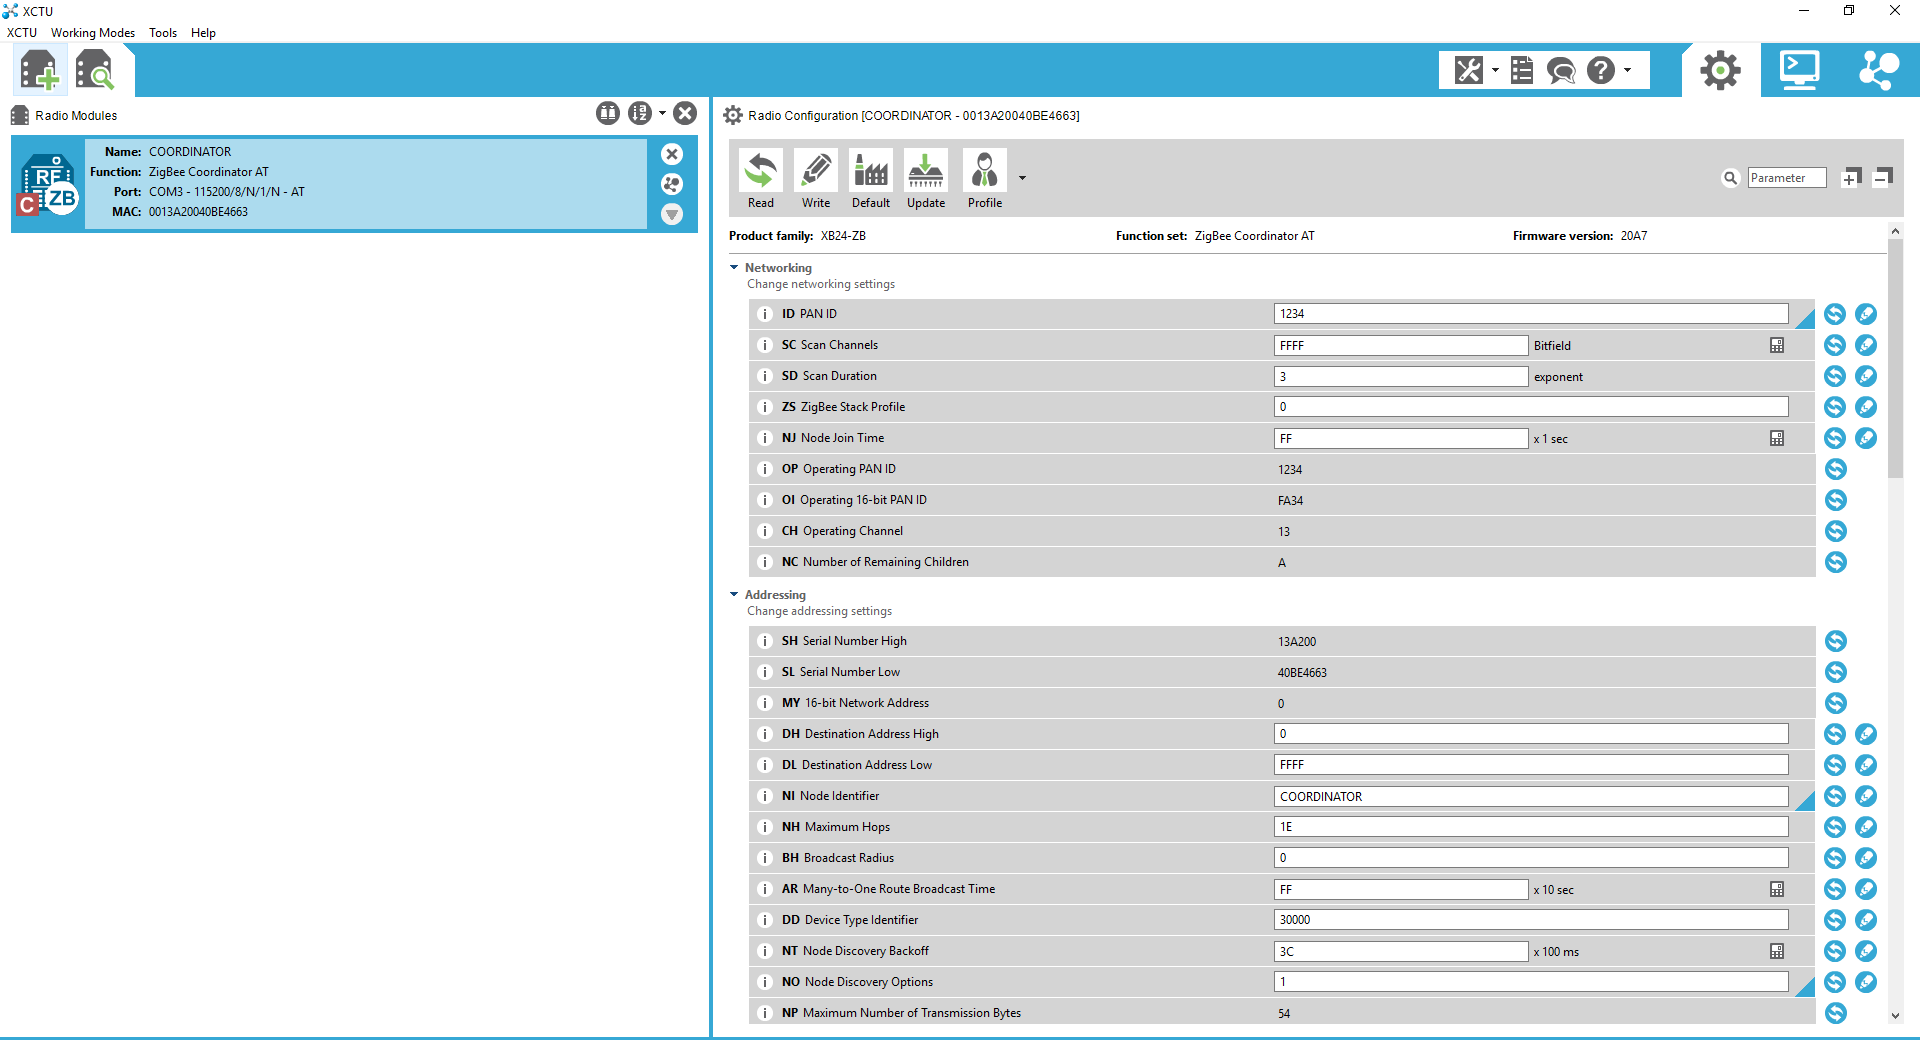
\includegraphics[width=0.9\textwidth, frame]{figuras/interfazXCTU.png}
\caption{Iterfaz de XCTU}
\label{fig:XCTU}
\end{figure}

Para cambiar el firmware, se puede hacer click en \textit{Update} (figura \ref{fig:firmXCTU}) y seleccionar un nuevo firmware y versión. Es en esta pantalla en la que se puede cargar firmware orientado a un modo de comunicación en concreto (AT o API). Al hacer click en Update comenzará el proceso de escritura del firmware y, tras unos segundos, el módulo estará listo para usarse. 

\begin{figure}[h]
\centering
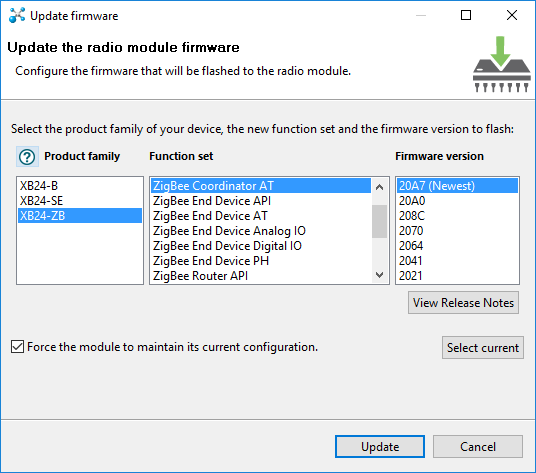
\includegraphics[width=0.5\textwidth]{figuras/firmXCTU.png}
\caption{Carga de firmware en XCTU}
\label{fig:firmXCTU}
\end{figure}

La interfaz de XCTU permite modificar multitud de parámetros que deben coincidir en todos los extremos de la comunicación. En la figura \ref{fig:XCTUPropCoord} se pueden observar los parámetros de configuración del XBee Coordinador AT, mientras que en la figura \ref{fig:XCTUPropRou} está la configuración del Router AT. En modo API son similares

\begin{figure}[H]
\centering
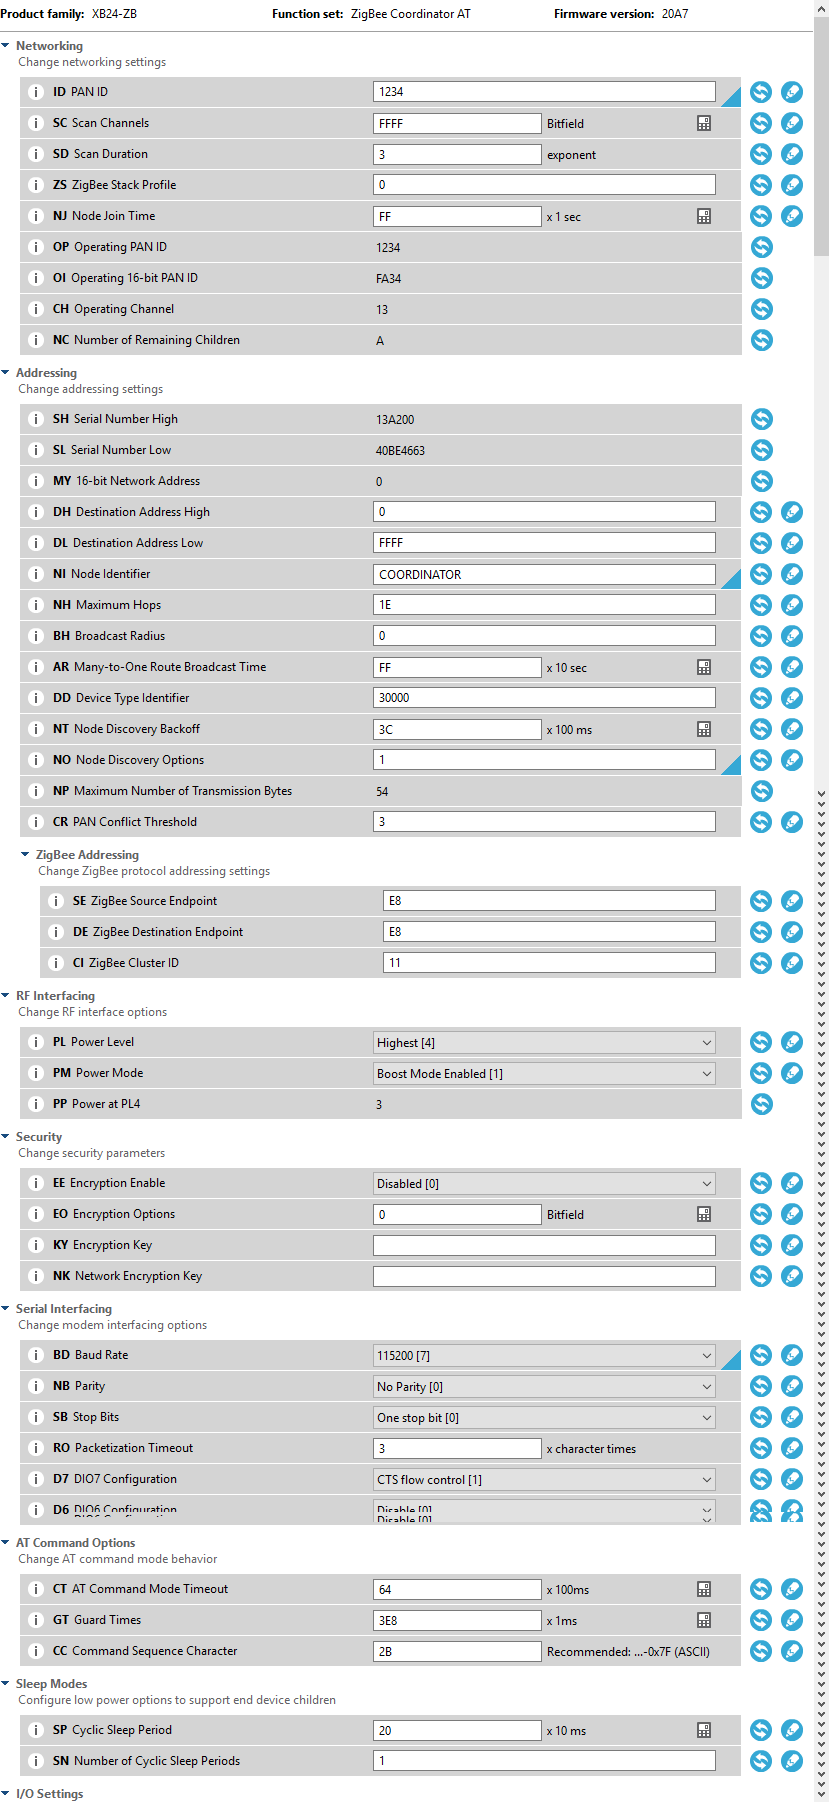
\includegraphics[width=0.75\textwidth]{figuras/XCTUPropCoord.png}
\caption{Propiedades del XBee Coordinador AT}
\label{fig:XCTUPropCoord}
\end{figure}

\begin{figure}[H]
\centering
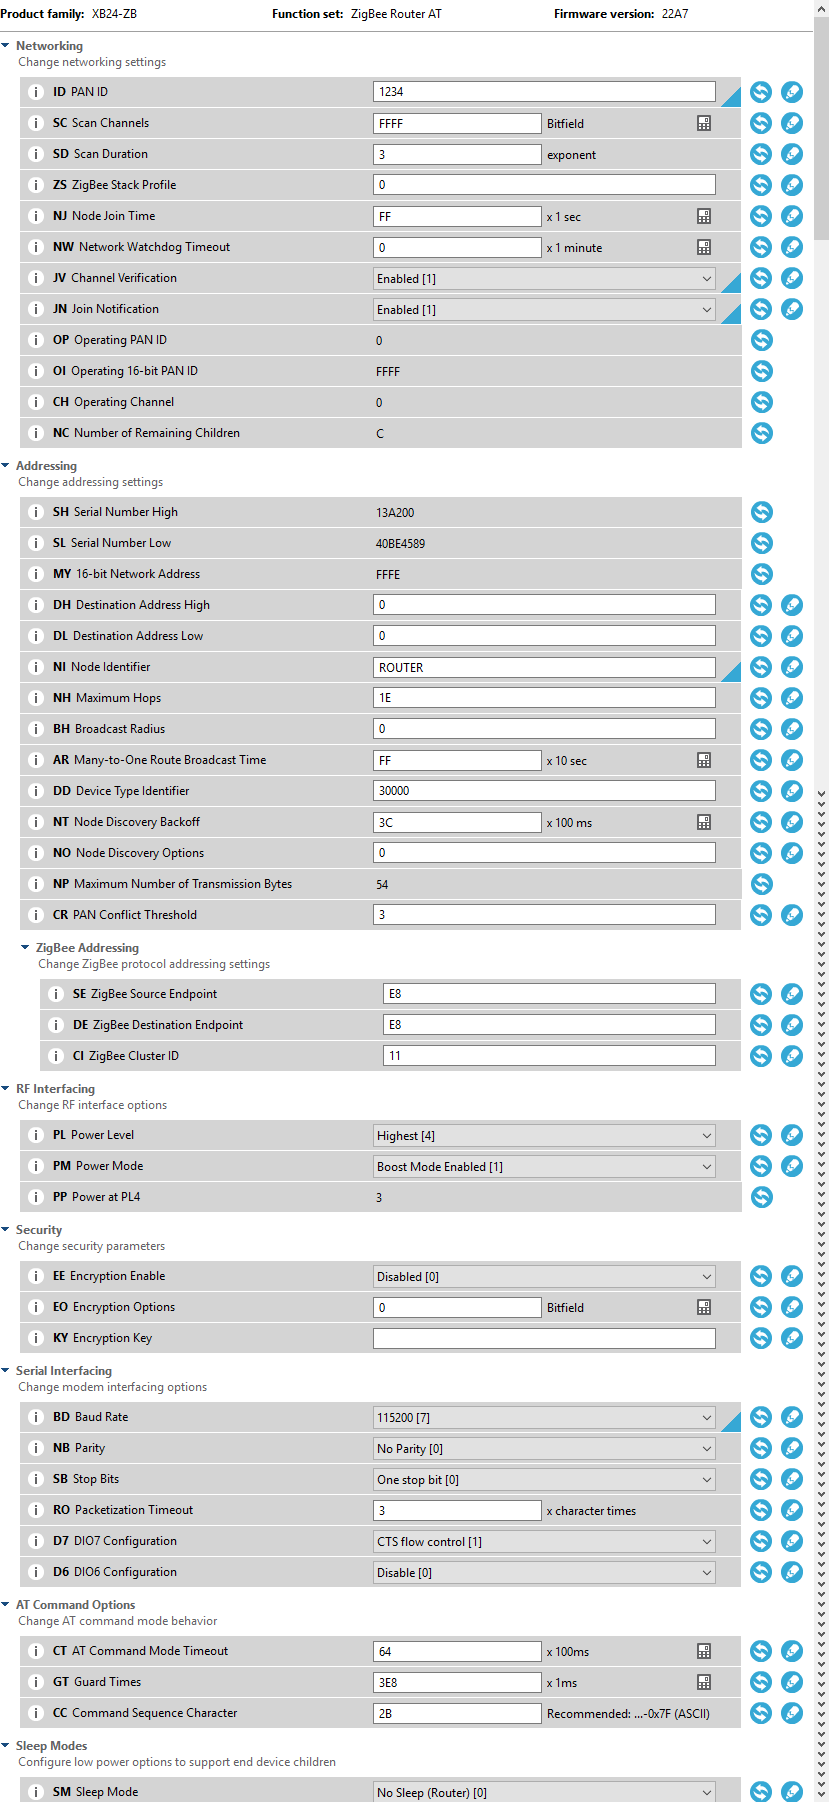
\includegraphics[width=0.75\textwidth]{figuras/XCTUPropRou.png}
\caption{Propiedades del XBee Router AT}
\label{fig:XCTUPropRou}
\end{figure}

Entre los parámetros configurables más destacables se encuentran los siguientes:

\begin{itemize}
\item \textbf{PAN ID} es el identificador de la red domótica.
\item \textbf{DH} y \textbf{DL} ponen límites a las direcciones entre las cuales el dispositivo transmitirá. Estas configuraciones a 0 en el router ponen al coordinador de la red como único destinatario.
\item \textbf{NI} es el nombre identificador del nodo.
\item \textbf{EE} maneja la posibilidad de encriptar la información para añadir una capa extra de seguridad.
\item \textbf{BD}, \textbf{NB} o \textbf{SB} son los parámetros correspondientes a la comunicación serial. En este caso, se sitúa la tasa de baudios en 115200, que es el máximo admitible por XCTU.
\end{itemize}

Por último, queda comentar la posibilidad de usar XCTU como terminal serie de manera sencilla y adaptada a la aplicación que estamos comentando. En la pestaña de consolo se puede consultar la emisión y recepción de cada módulo, como se muestra en la figura \ref{fig:XCTUconsola}.

\begin{figure}[bth]
\centering
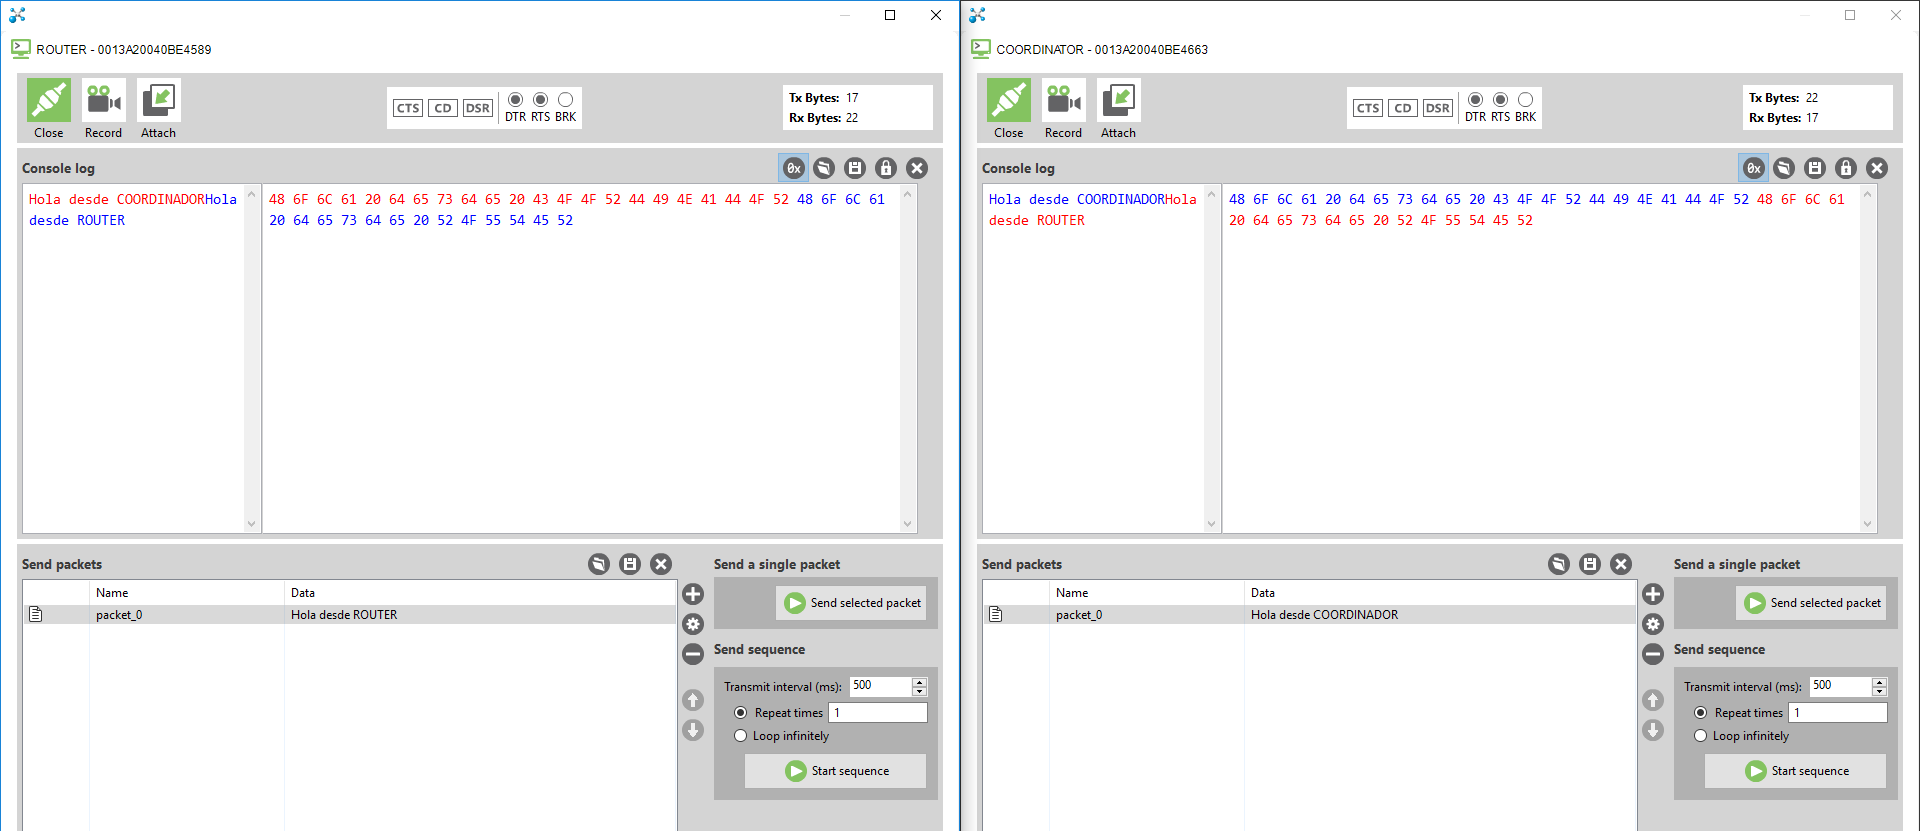
\includegraphics[width=1.1\textwidth, frame]{figuras/XCTUConsola.png}
\caption{Interfaz de consola de XCTU}
\label{fig:XCTUconsola}
\end{figure}


\subsection{Perfiles de comunicación}

La configuración introducida en XCTU se puede guardar y cargar de manera sencilla a través de la figura del perfil de comunicación. Estos perfiles son archivos que almacenan el firmware utilizado junto con toda la configuración específica.

Esto posibilita, como es el caso, la generación de los perfiles:

\textit{CoordinatorAPI.xpro}

\textit{RouterAPI.xpro}

\textit{CoordinatorAT.xpro}

\textit{RouterAT.xpro}

Siendo un proceso sencillo el de carga de un perfil a un módulo, es la manera más simple y rápida de cambiar el modo de comunicación de la red. No hay posibilidad de hacerlo sin cambiar el firmware.


\section{Modificaciones a RHA}

Se han realizado una serie de modificaciones al brazo robótico RHA con el fin de, por un lado, hacerlo compatible con las tecnologías usadas en este proyecto y, por el otro, solucionar algunos defectos que tenía.

En todo caso, la intención a lo largo del desarrollo del proyecto es obtener buenos resultados con una modificación mínima del estado inicial del brazo robótico, reduciendo al mínimo la posibilidad de generar incompatibilidades con futuros desarrollos ya planificados.

\subsection{Modificaciones Hardware}

Con modificaciones hardware se cuentan los cambios al proyecto inicial en cuanto a la configuración física, sensores o actuadores.

\begin{itemize}
\item El brazo robótico, de inicio, no tenía montado el mecanismo destinado al eje de rotación. Su funcionamiento era mejorable y este propósito se sale fuera del marco del presente proyecto, así que se decidió trabajar ignorando este eje.

\item El servo encargado de mover la articulación correspondiente al codo del RHA reportaba un error de sobrecarga aunque se le intentara hacer funcionar en vacío. La sensación al forzar la rotación sin alimentar el servo era muy diferente a la del otro servo que funcionaba correctamente, era mucho más difícil provocar esa rotación con la mano. Por todo esto, se concluyó que el servo estaba defectuoso y se sustituyó físicamente por el servo hasta ese momento encargado del movimiento del eje de rotación que se había definido como inutilizado.

\item Los potenciómetros no captaban de manera adecuada los movimientos de sus respectivos ejes. En el caso del codo, la pieza de impresión 3D que encajaba en el potenciómetro para rotarlo se había partido. En la articulación del hombro, la pieza de engranaje encargada de rotar el potenciómetro había cogido cierta holgura, provocando que no se generara rotación en la totalidad del movimiento del eje. En ambos casos se han solucionado los problemas mediante la utilización de un pegamento suficientemente fuerte.
\end{itemize}


\subsection{Modificaciones Software}

Teniendo en mente que la intención es reducir las modificaciones software lo máximo posible, solo se han hecho dos cambios de manera obligatoria.
\begin{itemize}
\item El defecto hardware que ha obligado a cambiar la posición de los servos tiene repercusiones en el software. Los servos no permiten otro orden de conexión más allá del previamente establecido. Más información sobre la comunicación del brazo con los servos puede encontrarse en el \cite{Heredia1:2018}/Anexo D. Si se cambia la posición física de los servos pero no se tocan sus conexiones, no hay más remedio que intercambiar la identificación de los servos en el software.

\item Como se ha mencionado en el apartado \ref{subsubsec:xctu}, la tasa de baudios máxima configurable para la comunicación serial de los módulos XBee es 115200. En el brazo robótico, la interfaz encargada de mandar frames de estado y recibir frames de comando trabajaba a 250000. Este dato también ha tenido que ser modificado para habilitar la comunicación, haciéndolo coincidir con el baudaje de los módulos XBee.
\end{itemize}

Por otro lado, y siendo un añadido al software, es necesaria la modificación de las funciones sendPackage() y receivePackage() para usar el modo API de comunicación. Al enviar un frame de información, este debe ser enmarcado en un API Frame de tipo 0x10 \textit{Transmit request} y eso es trabajo del software del brazo. En el mismo sentido va la modificación de la función encargada de la recepción de paquetes, debe esperarse la recepción de un API frame de manera previa a la recepción del frame propio de la comunicación con el RHA.

El código \ref{code:robot_rha_api} es un ejemplo de esto. Preprocesa el API frame antes de meterse a interpretar el frame de comandos RHA. Debe entenderse que es un else if tras un condicional que lee el inicio de un frame RHA. Es, por tanto, una alternativa no limitante de la lectura en modo transparente.

% Esto para configurar como se va a visualizar el código
\lstset{backgroundcolor=\color{amarillo_claro}, numbers=left,numberstyle=\tiny, language=C++, breaklines=true, basicstyle=\footnotesize, xleftmargin=25pt, framesep=8pt, numbersep=15pt}

\begin{lstlisting}[frame=leftline, caption={RHA API - getPackage()}, label=code:robot_rha_api]
else if (by1 == 0x7E)          //XBee comunication
{
    // Now a XBee msg can be read. XBee header was ok
    //Serial.println("XBEE");
    Serial_PYNTERFACE.read(); xbee_length = Serial_PYNTERFACE.read();
    uint8_t *data = new uint8_t[length];
    for(int k=0; k<length; k++) data[k]=Serial.read();
    if(data[0] == 0x90) {
        DebugSerialRRHALn("getPackage: Receive Packet");
    } 
    else {
        DebugSerialRRHALn("getPackage: Not supported Xbee frame");
        return;
    }
    
        if (data[12] == 0xFF && data[13] == 0xFF) {
            // Now a msg can be read. Header was ok
            DebugSerialRRHALn("getPackage: Header ok");
            Serial.println("getPackage: Header ok");
            length = data[14]; checksum += length;
            for (int k=0; k<length; k++) buffer_[k]=data[k+15];
            // Check if checksum is correct
            for (i = 0; i < length-1; i++) {
                checksum += buffer_[i];
            }
        checksum = ~checksum;
        // If its correct it can handle the information
        // Checksum is the last byte in package
        //if (readCount == length-1) { //} && checksum == buffer_[length]) {
        if (buffer_[0] == PynterfaceConstants::ARTICULAR_GOAL) {
            pynterface_goal_.x = buffer_[1];
            pynterface_goal_.y = buffer_[2];
            pynterface_goal_.z = buffer_[3];
            goToArticularPos(pynterface_goal_);
        }
    }
}
\end{lstlisting}


\section{Integración MQTT - Node-RED}

La conexión de los flujos de Node-RED con MQTT se realiza a través de unos nodos (figura \ref{fig:nodeMQTT}) desarrollados por terceros que ya han sido mencionados en el apartado \ref{subsec:nodered}.

El objetivo final de que MQTT esté integrado en Node-RED, es poder controlar toda la red domótica desde un dispositivo central (como una tablet) cuyo software únicamente interactúe con el topic en cuestión.

En el proyecto RoboHealth se han desarrollado dos flujos. Uno de ellos publica los estados de los dispositivos conectados a Vera y Zolertia 2 en el topic \textit{Robohealth/room/devices}; mientras que el otro está suscrito al mismo topic con la intención de actuar de acuerdo a los mensajes codificados que se publican.

Como se explicó en el apartado \ref{subsubsec:RH_MQTT}, cabe recordar que los mensajes para comandar dispositivos siguen el siguiente formato:

$$\{'id':xx,'atrib1':'yy','atrib2':'zz',(...)\}$$

Node-RED se encarga de añadir los atributos y sus valores al mensaje \textit{msg} para actuar en consecuencia. Usando el identificador 99, Robohealth Arm requiere de los atributos \textbf{shoulder} y \textbf{elbow}.

Así, por ejemplo, si se quiere comandar Robohealth Arm desde MQTT sólo será necesario publicar un mensaje como el siguiente en el topic \textit{Robohealth/room/devices}.

$$\{'id':99,'shoulder':'8C','elbow':'5A'\}$$

\subsection{Flujos MQTT}

En la actual sección se presentan los flujos de Node-RED que interactúan con MQTT, bien publicando en cierto \textit{topic} o subscribiéndose al mismo.

El flujo presentado en la figura \ref{fig:MQTTFlowR} muestra la etapa de suscripción. Está permanentemente a la escucha de las publicaciones de \textit{Robohealth/room/devices} y transforma el formato del mensaje MQTT en un objeto \textit{msg} propio de Node-RED gracias al \textit{nodo JSON}\footnote{Se trata de un nodo que ejecuta conversiones en ambos sentidos entre un string JSON (el mensaje de MQTT) y un objeto de JavaScript (el objeto \textit{msg} de Node-RED)}. El nodo Switch sirve para clasificar el mensaje en función de su identificador. A partir de ese punto, la acción es específica del dispositivo representado por el identificador recibido.

En el caso del brazo robótico, con identificador 99, se sitúa su salida en último lugar. La función \textit{Adapt msg} genera un \textit{msg.payload} compatible con el script sendAT.py (anexo \ref{anexo:sendAT}), que se ejecuta posteriormente.

\begin{figure}[hbt]
\centering
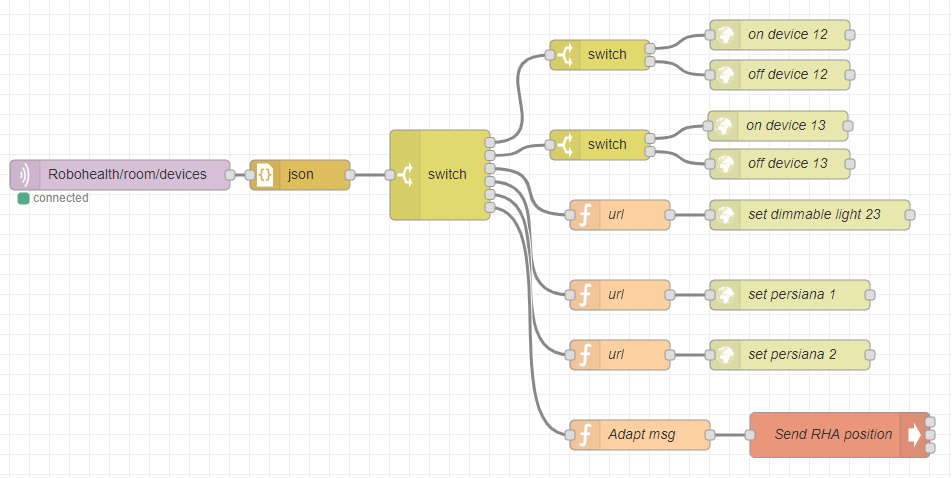
\includegraphics[width=0.9\textwidth]{figuras/MQTTFlowR.png}
\caption{Flujo de subscripción a MQTT}
\label{fig:MQTTFlowR}
\end{figure}

En la figura \ref{fig:MQTTFlowP} se muestra el flujo que publica en MQTT el estado de los dispositivos relacionados con la red Vera o con Zolertia 2 con fines informativos para los dispositivos suscritos al topic. 

\begin{figure}[hbt]
\centering
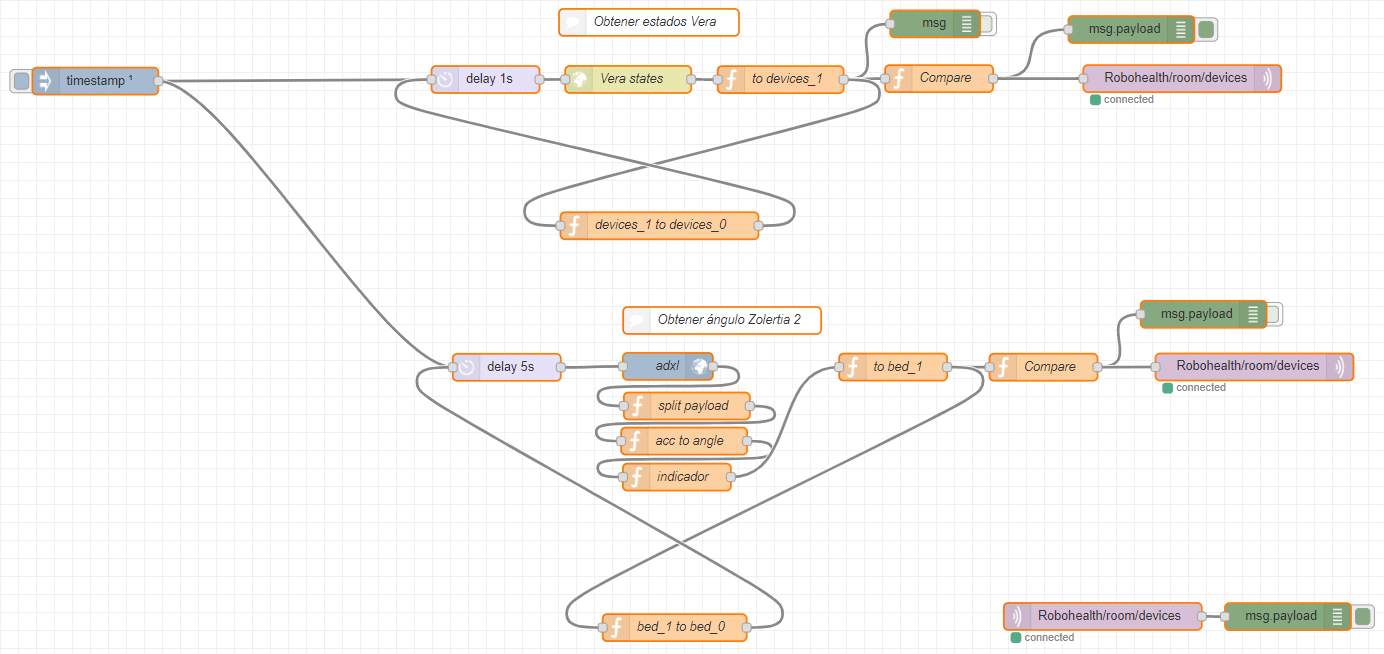
\includegraphics[width=0.9\textwidth]{figuras/MQTTFlowP.png}
\caption{Flujo de publicación en  MQTT}
\label{fig:MQTTFlowP}
\end{figure}

\section{Integración Node-Red - XBee}\label{subsec:NR-Xbee}

La integración de Node-RED con los módulos Xbee se realiza a través de comunicación serial comandada a través de los distintos scripts recogidos en el Anexo \ref{anexo:b}.

En Node-RED los scripts son llamados usando el nodo Exec (comentado en el apartado \ref{subsec:nodered}). Los nodos de envío se ejecutan rápidamente sin problemas y no generan salidas. El nodo de recepción, en cambio, permanece durante un tiempo indefinido volcando mensajes de estado del brazo robótico al flujo de Node-RED. Como inconveniente, comentar que no ha sido posible sacar las salidas correctas del programa por la salida estándar \textit{stdout} en Node-RED. Como se puede observar en el código \ref{code:Receive} y en el flujo de recepción de datos (figura \ref{fig:RecepcionRHA}, este problema se ha solucionado recurriendo a la salida de error \textit{stderr} que, en Node-RED, sí que funcionaba adecuadamente.

La comunicación serial se realiza con la configuración estándar (código \ref{code:SerialConf}), normalmente usada por defecto para la mayoría de dispositivos. Se establece, eso sí, una tasa de baudios de 115200 que, recordamos, era el máximo admisible por los módulos XBee

% Esto para configurar como se va a visualizar el código
\lstset{backgroundcolor=\color{amarillo_claro}, numbers=left,numberstyle=\tiny, language=Python, breaklines=true, basicstyle=\footnotesize, xleftmargin=25pt, framesep=8pt, numbersep=15pt}

\begin{lstlisting}[frame=leftline, caption={Configuración serial}, label=code:SerialConf]
ser = serial.Serial(
	port='/dev/ttyACM0',
	baudrate = 115200,
	parity=serial.PARITY_NONE,
	stopbits=serial.STOPBITS_ONE,
	bytesize=serial.EIGHTBITS,
	timeout=1
)
\end{lstlisting}

No es necesario hacer ninguna modificación a la información más allá de los scripts, por lo que la configuración hardware en modo USB de la XBee Shield encaja perfectamente en nuestras necesidades. Como se ha indicado previamente en el apartado \ref{subsubsec:USBXB}, es necesario retirar el microcontrolador del Arduino UNO y la unión funcionará como una conexión directa serie entre la Raspberry Pi y el módulo XBee Coordinador (figura \ref{fig:RPiXB}.

\begin{figure}[hbt]
\centering
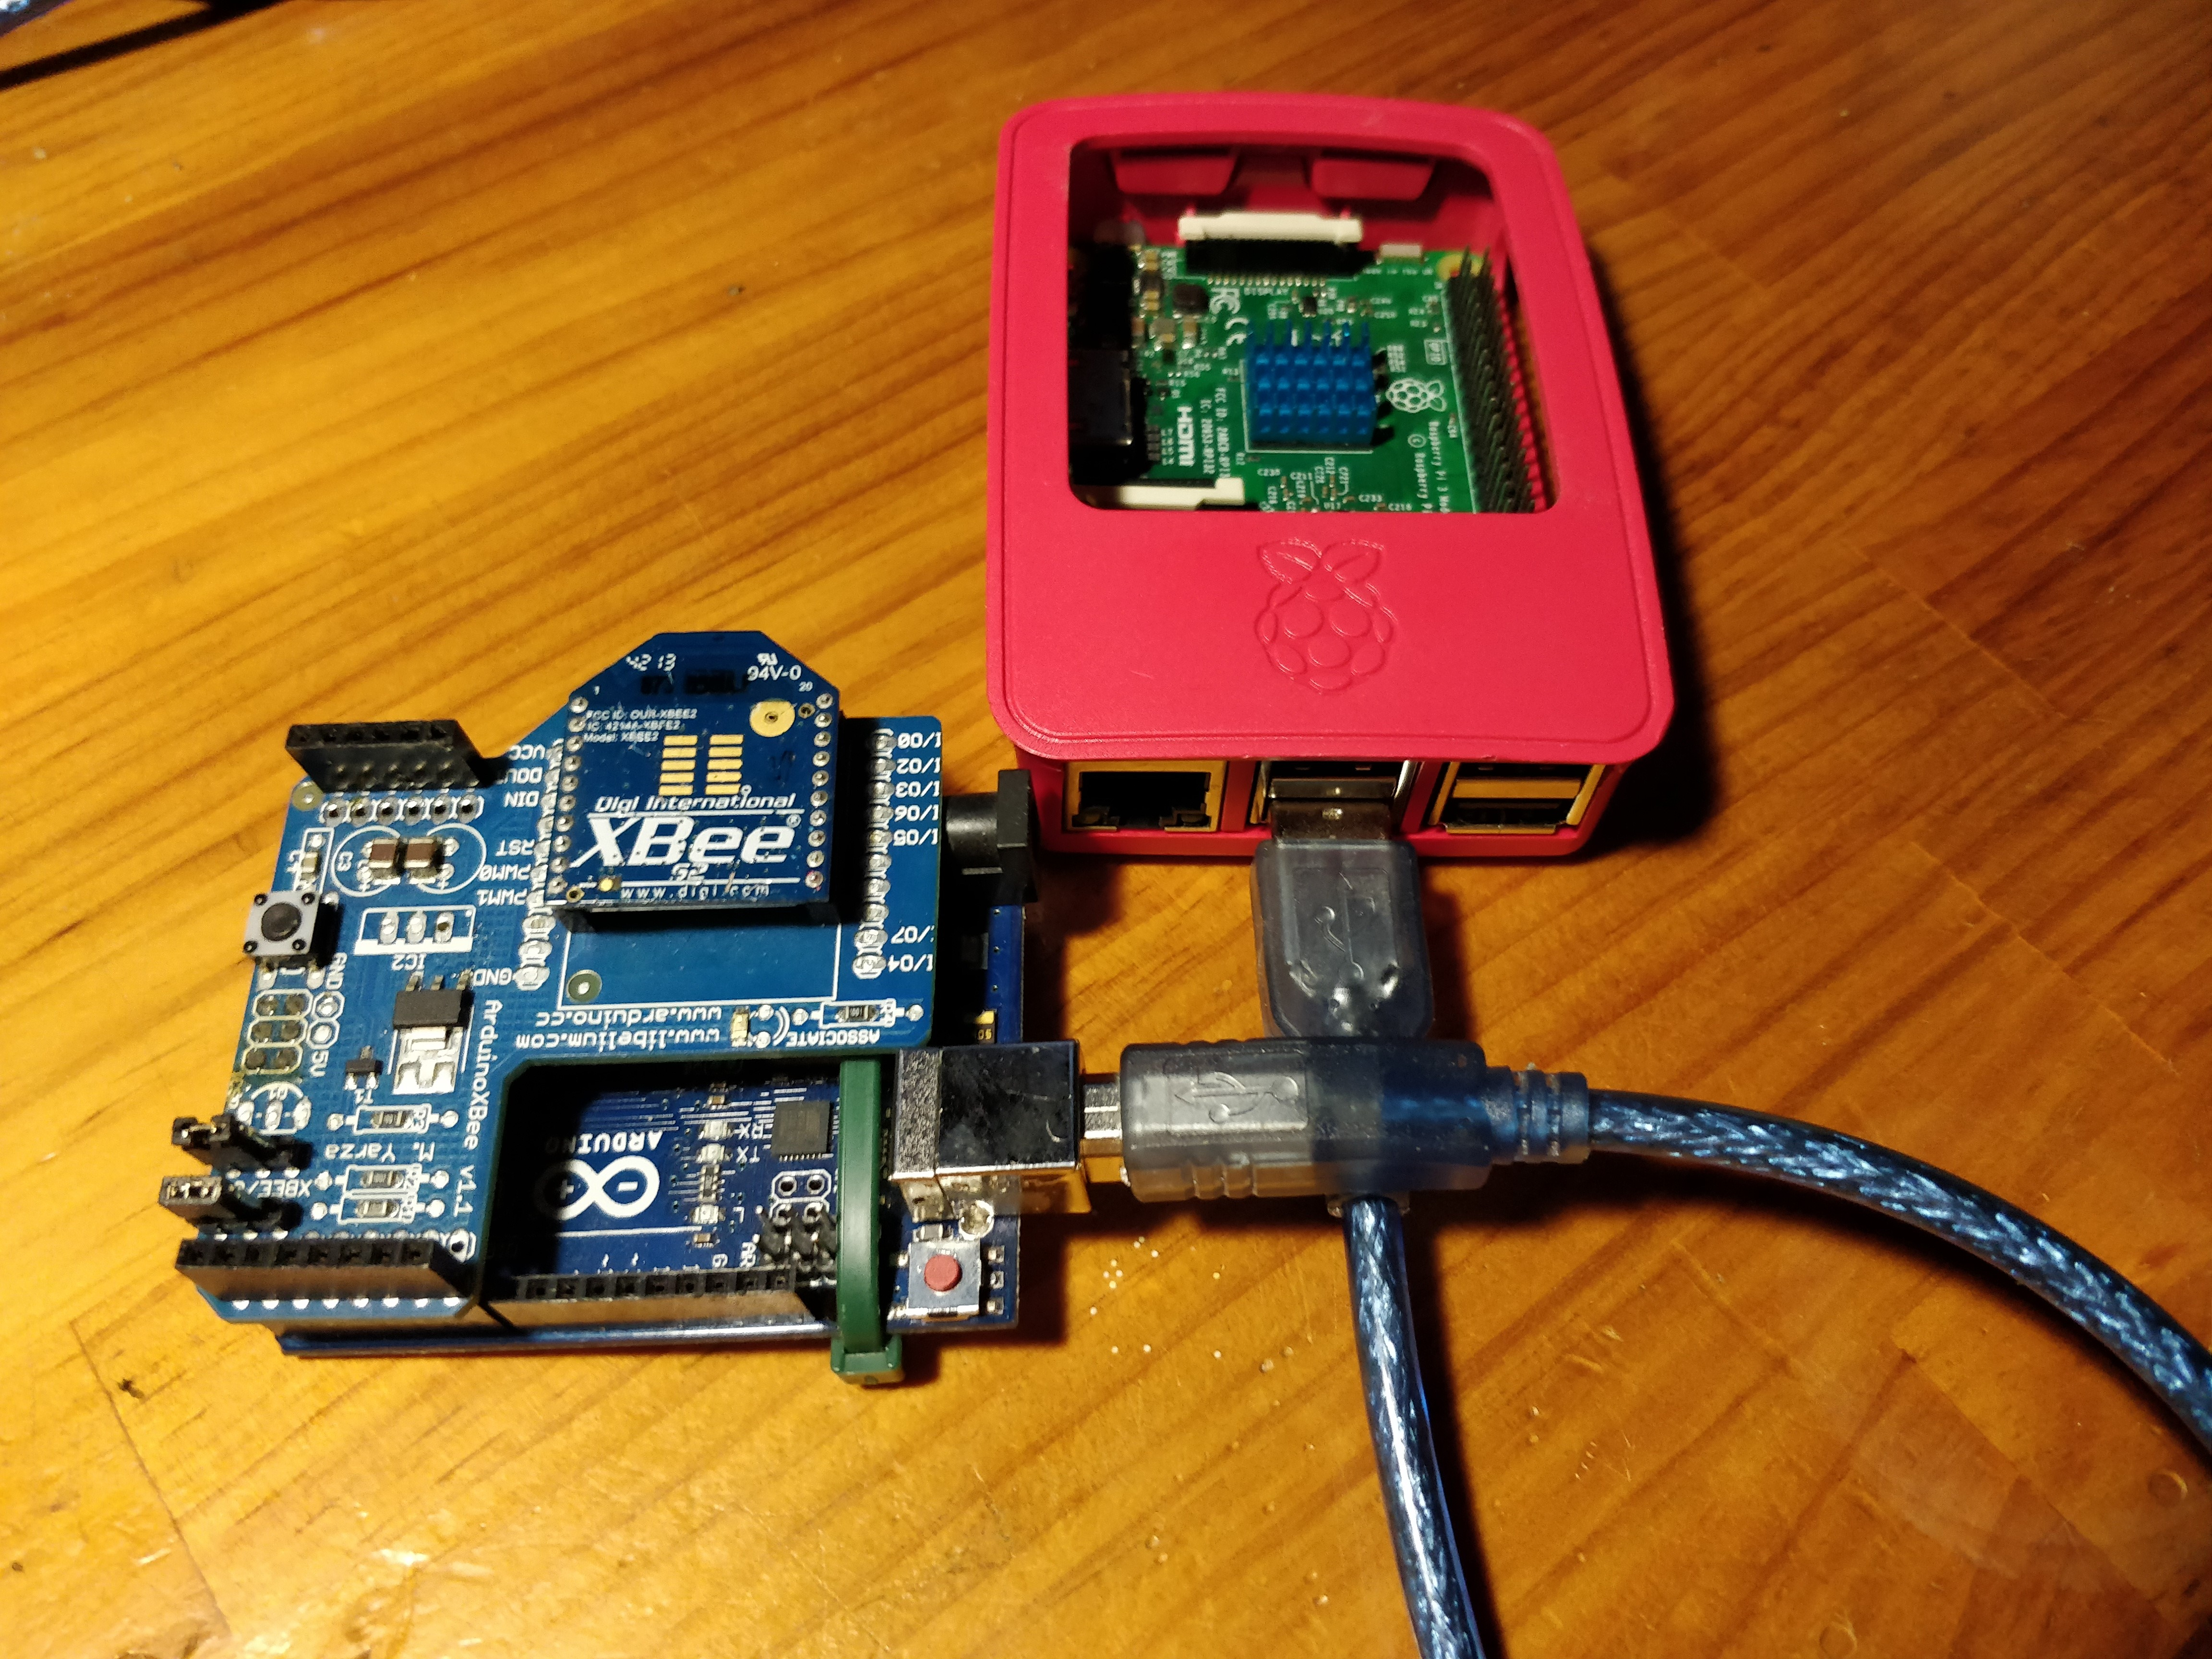
\includegraphics[width=0.6\textwidth]{figuras/RPiXB.png}
\caption{Conexión serial XBee-RPi}
\label{fig:RPiXB}
\end{figure}

También existe la posibilidad de conectar el módulo Xbee directamente usando los pines dedicados a comunicación serie del módulo y de la Raspberry Pi (figura \ref{fig:RPiXBserial}). Se ha optado por la primera solución porque esta segunda va a ser la aplicada en el siguiente apartado y por facilitar en montaje y la conexión en el lado de la unidad de mando. 

\begin{figure}[hbt]
\centering
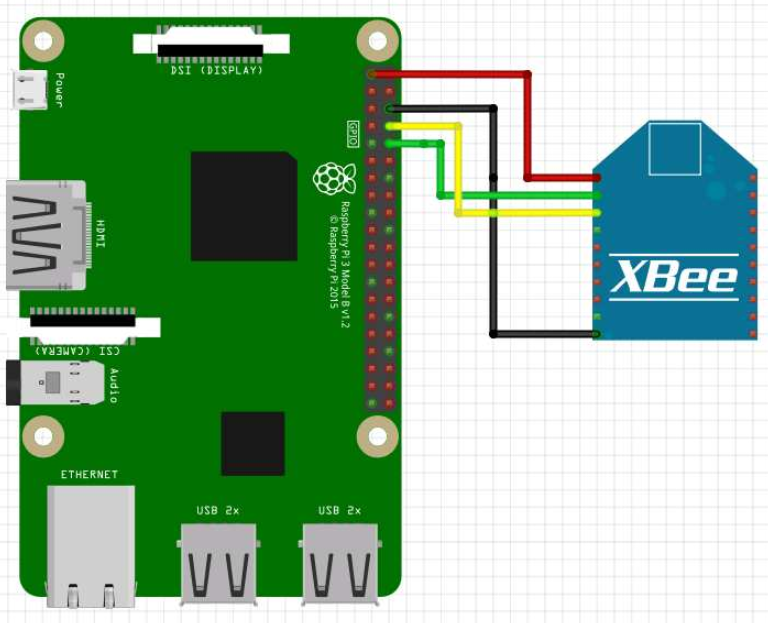
\includegraphics[width=0.5\textwidth]{figuras/RPiXBserial.png}
\caption{Conexión serial alternativa XBee-RPi}
\label{fig:RPiXBserial}
\end{figure}

\section{Integración XBee - RHA}

Por su parte, no hay otra opción para conectar el módulo XBee al Arduino Mega del RoboHealth Arm que usar los pines seriales. Estos pines son, en el módulo XBee, DOUT y DIN y, en el Arduino Mega, D0(RX) y D1(TX)\footnote{El Arduino Mega posee otros tres puertos seriales que podrían ser igualmente usados}. El diagrama de conexiones se muestra en la figura \ref{fig:AMegaXBserial}. Existe la posibilidad de usar alguno de los dos puertos seriales restantes\footnote{Uno de los tres está usado por los servos} para evitar cualquier potencial interferencia en la comunicación por el USB pero esto implicaría modificar el código cambiando el puerto serial de la interfaz \textit{Pynterface}.

\begin{figure}[hbt]
\centering
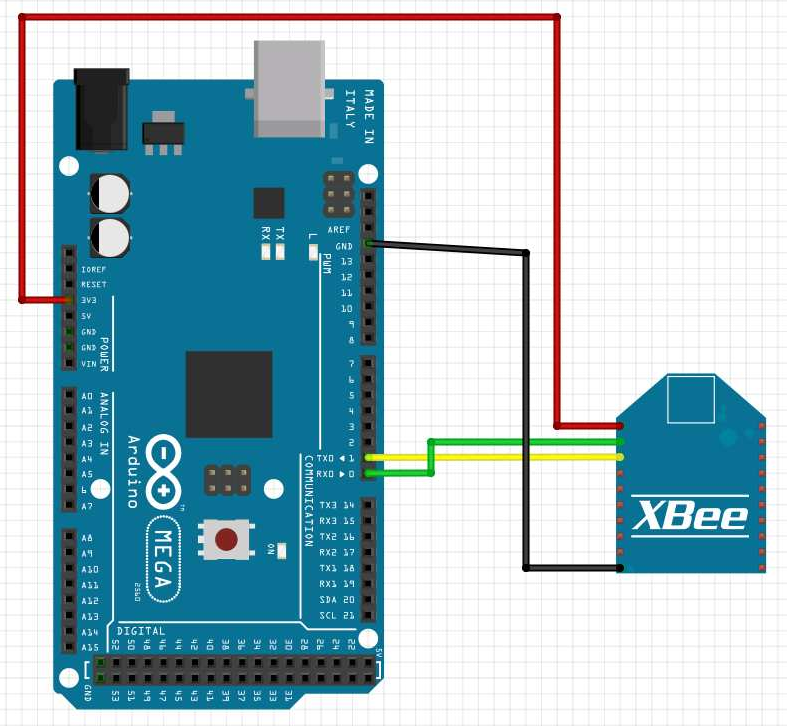
\includegraphics[width=0.5\textwidth]{figuras/AMegaXBserial.png}
\caption{Conexión serial Arduino Mega - XBee}
\label{fig:AMegaXBserial}
\end{figure}